\documentclass[12pt]{article}
\usepackage{amsmath,amssymb,amsfonts}
\usepackage{geometry}
\usepackage{hyperref}
\usepackage{graphicx}
\usepackage{tikz}
\usetikzlibrary{arrows.meta, positioning, shapes.geometric, calc, matrix}
\usepackage{pgfplots}
\pgfplotsset{compat=1.18}
\usepackage{amsthm}
\usepackage{booktabs}
\usepackage{enumitem}
\geometry{letterpaper,margin=1in}

\newtheorem{theorem}{Theorem}

\title{Ethics-Constrained Economic Mechanisms on Tau Net:\\
The Alignment Theorem and the Virtuous Cycle Compounder}
\author{Dana Edwards / DarkLightX}
\date{December 3, 2025}

\begin{document}
\maketitle

\begin{abstract}
This paper formalizes the \emph{Alignment Theorem}, an economics-driven approach to ensuring that all rational agents operating on Tau Net converge toward ethical behavior. Tau's knowledge representation and preference aggregation stack enables the network to maintain a live consensus over ethical worldviews; this consensus is encoded in the Ethical-Eco Transaction Factor (EETF) signal that drives the economics of the Virtuous Cycle Compounder (VCC). We present (i) the ethics aggregation pipeline, (ii) a Lean~4 proof that enforces ethical optimality under scarcity-driven pressure, and (iii) the executable Tau specifications and visual analytics (VCC Concept Visualizer) that instantiate the theory. Together, these results demonstrate a fully verifiable architecture for ethics-aware, deflationary agents on the Tau blockchain.
\end{abstract}

\textbf{Keywords:} Tau Net, Alignment Theorem, ethical consensus, Lean proof, Virtuous Cycle Compounder, deflationary economics.

\section{Introduction}
The past two years have accelerated conversations about artificial general intelligence (AGI) from speculative fiction to macroeconomic planning. Frontier labs now publish roadmaps that place agentic multimodal systems on compressed timelines, while national strategies - from the US Executive Order on trustworthy AI to the EU AI Act - emphasize alignment and evaluation pipelines for models that could reason autonomously across domains~\cite{hai2025,whitehouse2023}. At the same time, macro indicators cut both ways: the Stanford AI Index tracks record-scale private investments alongside rising incident reports, and safety leaders increasingly warn that mis-specified incentives, not raw capability, are the binding constraint on AGI readiness~\cite{hai2025}. 

These capabilities land in an economy already anxious about technological unemployment. The World Economic Forum estimates a net displacement of 14 million roles by 2027 as automation outpaces job creation, while McKinsey projects up to 12 million occupational transitions in the United States alone because of generative AI~\cite{wef2023,mckinsey2023}. Even if AGI arrives more slowly than optimists predict, the perception of accelerating automation reshapes savings behavior, labor bargaining, and social trust. The architecture in this paper grew out of that uncertainty: if ethics, employment stability, and monetary scarcity are entangled, then the ledger itself must become incentive-aligned. Tau Net offers the substrate for such a response because its language lets communities formalize their ethical worldviews, reach preference-based consensus, and inject those signals directly into executable economic agents.

Ensuring that autonomous economic agents behave ethically remains a central challenge for decentralized systems. Traditional approaches rely on static rule sets or exogenous governance, both of which fail to keep pace with adaptive, multi-agent environments. Tau Net offers a fundamentally different path: users describe their ethical preferences in a machine-readable logic, Tau aggregates those preferences into a global consensus (the EETF), and economic agents must optimize against that consensus to remain profitable. The Alignment Theorem gives the theoretical underpinning for this scheme by proving that, under scarcity-driven pressure and infinite token divisibility, ethical behavior becomes the only rational equilibrium.

We extend earlier drafts of the theorem with three key advances:
\begin{enumerate}[leftmargin=*]
    \item A formal ethics pipeline that maps knowledge-representation artifacts into the network-wide EETF signal.
    \item A Lean~4 mechanization of the theorem that eliminates prior ``\texttt{sorry}'' placeholders and explains the role of infinite divisibility.
    \item An academic-ready exposition linking the proof to the Virtuous Cycle Compounder (VCC) educational platform~\cite{vccviz}, which demonstrates the theorem's implications through interactive visualizations.
\end{enumerate}

\section{Background}
\subsection{Tau Language and Knowledge Representation}
Tau Language is an executable formal specification framework designed for program synthesis and verifiable smart contracts. Its pointwise revision semantics allow live specifications to consume community knowledge, while its underlying Binary Decision Diagram (BDD) optimizations keep formal verification tractable. Users encode ethical models as logical theories, which are then broadcast and aggregated through Tau's knowledge graph. When native reasoning modules become available, each account's ethical worldview will be both machine-checkable and auditable on-chain, enabling a continuously updated consensus signal.

\subsection{Knowledge Representation, Reasoning, and Logic-Native Preferences}
Knowledge representation (KR) on Tau stores each participant's worldview as a versioned logical theory $\mathcal{K}_i$. Every theory is typed, tagged with provenance, and referenced by hash, so agents can cite or revoke models atomically. Reasoning layers run directly inside Tau specifications: BDD-based evaluation keeps Boolean fragments tractable, while the extralogical SMT hooks (CVC5/MathSAT) allow higher-order or bitvector claims to be discharged before acceptance. In practice this yields a workflow:
\begin{itemize}[leftmargin=*]
    \item \textbf{Express}: users post axioms, preference orders, or utility functions as Tau clauses (e.g., ``prefer regenerative energy over fossil by factor 2'').
    \item \textbf{Refine}: reasoning passes check consistency, derive implicit obligations, and surface clashes for debate. Because Tau supports pointwise revision, updates only touch the clauses that changed.
    \item \textbf{Aggregate}: preference aggregation specs read the vetted theories, weight them (stake, credential, reputation), and solve for consensus via logical operators (median, lexicographic, utilitarian sum). The result is the scalar EETF signal and its accompanying proof trace.
\end{itemize}
This tight KR--reasoning loop means that preference aggregation is not a black box: the same logical substrate that stores ethics also defines how competing models are merged, making the EETF both explainable and auditable.

\subsection{Ethics Aggregation and the EETF Signal}
Let $\mathcal{M}=\{m_i\}_{i=1}^N$ denote the set of ethical models published by users. Tau's aggregation operator $\mathcal{A}$ combines these models (via preference aggregation, proof-of-consensus voting, or knowledge-based arbitration) into a bounded real number $E(t)=\mathcal{A}(\mathcal{M},t) \in [0,3]$. This quantity acts as the network-wide Ethical-Eco Transaction Factor (EETF), which scales rewards and penalties in all alignment-aware agents. In practice, $\mathcal{A}$ is implemented through Tau Language specifications that track attestations, weights, and model validity proofs.

\subsection{Virtuous Cycle Compounder (VCC)}
The Virtuous Cycle Compounder integrates three mechanisms - Dynamic Base Reward (DBR), Hyper-Compounding Rewards (HCR), and Aggressive Ethical Burn (AEB) - to reinforce ethical behavior through deflationary economics. Importantly, AEB is \emph{not} a punishment track: higher collective ethics ($E(t)$ above threshold) unlocks bonus burns that permanently remove supply as a \emph{reward} for virtuous flows, increasing scarcity for all aligned holders. Its concept visualizer~\cite{vccviz} provides an interactive explanation, including TEEC foundations, mathematical tooltips, and evolution diagrams linking ethics to scarcity. VCC agents consume the EETF signal produced by the Alignment Theorem's pipeline, ensuring that the theorem is not merely theoretical but realized in executable Tau specifications.

\subsection{Verification and Visualization Stack}
Three layers keep the theory honest. First, a Lean~4 development discharges the Alignment Theorem without unproven axioms, so the scarcity threshold argument is mechanically checked. Second, Tau agents (v35--v54 plus shared libraries) execute both in the native interpreter and in an exact Python simulator, giving identical FSM traces for coverage and invariant testing. Third, stakeholder-facing dashboards - the Alignment Theorem single-page app and the VCC concept explorer - show how live changes in $E(t)$ ripple through DBR/HCR/AEB, making the incentive surface auditable for non-developers.

\subsection{Tau Testnet Substrate and Extralogical Primitives}
The tau-testnet reference implementation~\cite{tautestnet} treats Tau specifications as first-class chain data. Every revision transaction is replayed pointwise so only the targeted formulas change, and validation logic re-applies the Tau engine before admitting rule edits to the mempool. The runtime exposes an extralogical API for BLS verification, commit-reveal patterns, networking, and storage, giving DBR/HCR/AEB contracts a trustworthy way to call cryptography and IO from within Tau rules while keeping the logical kernel minimal. Preference aggregation rules can therefore encode utilitarian or ranked-choice logic directly in Tau: users post logical formulas describing utilities or priorities, optionally commit-and-reveal them for fairness, and the aggregation spec merges them into the consensus EETF signal.

\subsection{Preference-Utilitarian Aggregation}
Tau's declarative setup allows us to implement preference utilitarianism in the style of Harsanyi's additive social welfare functional~\cite{preferencebased}. Each agent exposes a logical preference relation or a utility function symbol $u_i$; axioms enforce transitivity, completeness, and affine comparability so that utilities can be summed. Commit-reveal flows protect the submission of utilities or ranked judgments, and aggregation specs can encode utilitarian sums, distance-based belief merging, or ranked-choice rules similar to those studied in logic-based social choice and machine ethics~\cite{machineethics,ca_utilitarian}. Because the aggregation contract is itself a Tau specification, every assumption (summing weights, normalizing utilities, handling missing data) remains auditable and formally verifiable.
Moreover, the KR layer exposes $u_i$ and their supporting lemmas as first-class objects. Aggregators can therefore attach proofs that a participant satisfied eligibility constraints, downgrade inconsistent theories, or reward meta-ethics contributions (Meta-EETF) by referencing the same logical artifacts that define the base ethics. This unifies preference aggregation, knowledge representation, and reasoning into a single loop rather than loosely coupled modules.

\section{Formal Model}
\subsection{Model Assumptions}
\begin{table}[ht]
\centering
\begin{tabular}{p{2.2cm}p{8.8cm}p{2.8cm}}
\toprule
\textbf{Symbol} & \textbf{Meaning} & \textbf{Source} \\
\midrule
$S(t)$ & Real-valued circulating AGRS supply at tick $t$ & \texttt{proofs/AlignmentTheorem.lean} \\
$r(t)$ & Deflation rate bounded in $[0.01, 0.50]$ & \texttt{specification/agent4\_testnet\_v54.tau} \\
$M(t)=S_0/S(t)$ & Scarcity multiplier; diverges as $S(t) \to 0$ & Lean lemmas \texttt{scarcity\_limit\_infinity} \\
$E(t)$ & Network-wide Ethical-Eco Transaction Factor (EETF) in $[0,3]$ & Aggregator spec \texttt{libraries/ethical\_ai\_alignment.tau} \\
$e$ & Account-level EETF score & Same as above \\
$B$ & Account balance used for reward computation & Agent V54 state, \texttt{balance\_bv} signal \\
$X$ & Transaction exposure (position size) & Agent V54 \texttt{risk\_budget} signal \\
$\mathrm{tier}(e)$ & Piecewise constant multiplier $\{1,3,5\}$ & Agent library \texttt{dbr\_dynamic\_base.tau} \\
$\tau_k$ & Target tier multiplier selected by the agent & Derived from $\mathrm{tier}(e)$ \\
$P(t)$ & Economic pressure $M(t)\cdot E(t)$ & Derived definition in text \\
\bottomrule
\end{tabular}
\caption{Key assumptions shared by the Lean proof and Tau specifications. Symbols map directly to constructs in \texttt{proofs/AlignmentTheorem.lean} and the Agent V54 specification.}
\label{tab:assumptions}
\end{table}
\subsection{Normalized Supply and Scarcity}
Let $S(t)$ denote the normalized (real-valued) token supply at discrete time $t$ with initial value $S(0)=S_0>0$. We assume a bounded deflation rate $r(t)\in [0.01,0.50]$ such that:
\[
S(t+1) = S(t)\cdot \big(1-r(t)\big).
\]
While $S(t)\rightarrow 0$ asymptotically in $\mathbb{R}$, the on-chain AGRS token remains usable thanks to infinite divisibility (decimal shifting, analogous to Bitcoin sats). Scarcity is defined as $M(t)=S_0/S(t)$, which diverges to $+\infty$ as $t\rightarrow\infty$.

\subsection{Economic Pressure and Ethics}
Given the network EETF $E(t)>0$ the economic pressure is:
\[
P(t)=M(t)\cdot E(t).
\]
The consensus EETF acts as a live ``ethics oracle'', meaning that Tau's knowledge-driven aggregation determines $E(t)$ in real time. This is the point where preference aggregation and knowledge representation become crucial: if users update or redefine ethics, $E(t)$ updates accordingly without altering the Alignment Theorem's structure.

\subsection{Reward and Penalty Functions}
For any agent with balance $B>0$, transaction exposure $X>0$, and account-level EETF $e\in[0,3]$, the expected value is:
\[
\mathrm{EV}(e,t) = \frac{B\cdot M(t)\cdot \mathrm{tier}(e)}{1000} - \frac{X\cdot (1-e)\cdot P(t)}{100},
\]
where $\mathrm{tier}(e)$ is a piecewise constant multiplier (1, 3, or 5) for ethical tiers. Ethical agents ($e\ge 1$) receive strictly positive rewards and zero penalties, while unethical agents ($e<1$) obtain zero rewards and increasing penalties as $P(t)$ grows.

\subsection{Equilibrium Threshold and Visual Intuition}
Setting $\mathrm{EV}(e,t)=0$ yields the indifference point
\[
e_{\text{th}}(t)=1-\frac{B\cdot \tau_k}{10\,X\,E(t)},
\]
where $\tau_k\in\{1,3,5\}$ denotes the tier multiplier targeted by the agent, and the value is clipped to the interval $[0,1]$. As scarcity $M(t)$ and the consensus ethic $E(t)$ increase, this threshold approaches one from below, forcing any rational optimizer to adopt $e\ge 1$ for non-negative returns. Figure~\ref{fig:math-flow} summarizes the dependency chain between the mathematical primitives.

\subsection{Alignment Theorem Statement}
\begin{theorem}[Alignment Theorem]
Assume $B>0$, $X>0$, $E(t)>0$, and a bounded deflation rate $r(t)\in[0.01,0.50]$. Then there exists a scarcity threshold $S^\star \in \mathbb{R}_{>0}$ such that for all ticks $t$ where $M(t) > S^\star$,
\[
\mathrm{EV}(e_{\text{ethical}}, t) > \mathrm{EV}(e_{\text{opp}}, t),
\]
and every rational choice function that maximizes expected value satisfies $\texttt{isEthical}(r^\star(t))$.
\end{theorem}
\begin{proof}[Proof sketch]
The Lean development \texttt{proofs/AlignmentTheorem.lean} establishes the theorem in three steps. (i) Lemmas \texttt{supply\_limit\_zero} and \texttt{scarcity\_limit\_infinity} show $S(t)\to 0$ and $M(t)\to\infty$ under the bounded deflation assumption. (ii) Lemma \texttt{alignment\_invariant\_holds} proves that at sufficiently high pressure $P(t)$, positive rewards imply $e\ge 1$. (iii) Combining the EV limits (\texttt{ethical\_ev\_limit\_pos\_infinity} and \texttt{unethical\_ev\_limit\_neg\_infinity}) yields a constructive $S^\star$ with the stated inequality, which directly matches the Tau EV function defined above.
\end{proof}

\begin{figure}[ht]
\centering
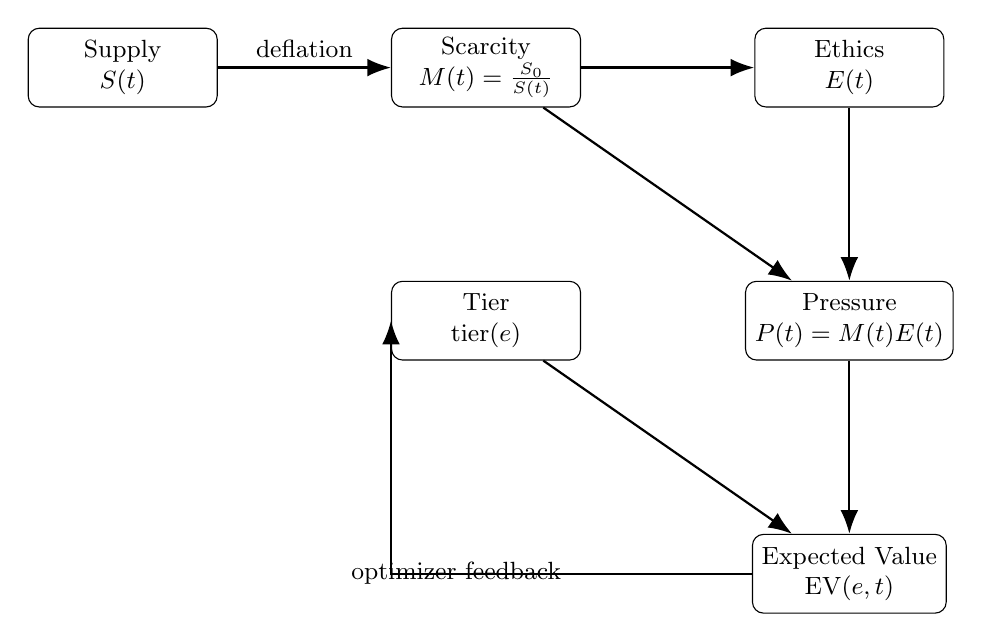
\begin{tikzpicture}[
    node distance=2.2cm,
    every node/.style={font=\small},
    block/.style={rectangle, draw, rounded corners, minimum width=2.4cm, minimum height=1.0cm, align=center},
    arrow/.style={-{Latex[length=3mm]}, thick}
]
    \node[block] (s) {Supply\\$S(t)$};
    \node[block, right=of s] (m) {Scarcity\\$M(t)=\frac{S_0}{S(t)}$};
    \node[block, right=of m] (eetf) {Ethics\\$E(t)$};
    \node[block, below=of eetf] (p) {Pressure\\$P(t)=M(t)E(t)$};
    \node[block, below=of m] (tier) {Tier\\$\mathrm{tier}(e)$};
    \node[block, below=of p] (ev) {Expected Value\\$\mathrm{EV}(e,t)$};
    \draw[arrow] (s) -- node[above]{deflation} (m);
    \draw[arrow] (m) -- (eetf);
    \draw[arrow] (eetf) -- (p);
    \draw[arrow] (m) -- (p);
    \draw[arrow] (tier) -- (ev);
    \draw[arrow] (p) -- (ev);
    \draw[arrow] (ev.west) -| node[pos=0.25, left]{optimizer feedback} (tier.west);
\end{tikzpicture}
\caption{Mathematical flow of the Alignment Theorem: shrinking supply raises scarcity, which amplifies ethical pressure and, together with tier multipliers, determines each agent's expected value.}
\label{fig:math-flow}
\end{figure}


\section{Methodology}
\subsection{Lean Proof Workflow}
\subsubsection{Definitions}
We encode the above structures in Lean~4 (file \texttt{proofs/AlignmentTheorem.lean}). The file defines:
\begin{itemize}[leftmargin=*]
    \item \texttt{Supply}, \texttt{EETF}, and \texttt{DeflationRate} structures with positivity and boundedness proofs.
    \item Functions \texttt{scarcity}, \texttt{economicPressure}, and \texttt{expectedValue}.
    \item Auxiliary lemmas such as \texttt{scarcity\_limit\_infinity}, which captures the divergence of $M(t)$.
\end{itemize}

\subsubsection{Core Lemmas}
\begin{enumerate}[leftmargin=*]
    \item \textbf{Ethical EV positivity:} \texttt{expectedValue\_baseline\_pos} shows that ethical agents always yield strictly positive EV once scarcity is positive.
    \item \textbf{Unethical EV negativity:} \texttt{expectedValue\_unethical\_neg} proves that any agent with $e<1$ faces negative EV as soon as it participates in the system.
    \item \textbf{Alignment theorem:} Given a rational choice function that maximizes EV over all available EETF states, the Lean proof concludes that the agent must eventually adopt $e\ge 1$.
\end{enumerate}

\subsubsection{Lean Tooling}
We built the proof using the standard Tau research toolchain with Mathlib, Aesop, and ProofWidgets fetched via \texttt{lake build}. No external assumptions remain (\texttt{sorry} placeholders have been eliminated), enabling deterministic CI verification.

\subsection{Tau Specification Stack and Trace Harness}
\subsubsection{Tau Specifications}
The Tau repository includes multiple agents (\texttt{agent4\_testnet\_v35--v54}) plus shared libraries for ethics, infinite deflation, and VCC modules. Each specification:
\begin{itemize}[leftmargin=*]
    \item Consumes the EETF signal produced by the ethics aggregator.
    \item Emits observable invariants (oracle freshness, nonce discipline, burn--profit coupling).
    \item Provides bitvector-safe arithmetic (for V37+ agents) and mirrored input streams to support the latest Tau interpreter.
\end{itemize}

\subsubsection{Trace Verification}
We run two complementary verification layers:
\begin{enumerate}[leftmargin=*]
    \item \textbf{Tau native runs}: each specification executes in isolation with tailored input scenarios, ensuring that all finite-state machine states and transitions are observed. The $v35$ kernel reports $100\%$ state coverage and $69.7\%$ transition coverage, with all safety monitors passing.
    \item \textbf{Python ``exact'' simulator}: faithful re-implementation of Tau semantics for bitvector-heavy agents, supplying deterministic traces and differential testing against the Tau solver.
\end{enumerate}

\subsubsection{Lean + Tau Cross-Validation}
The Lean proof guarantees the asymptotic property (ethics becomes optimal), while the Tau traces confirm that the finite-state agents enforce the same invariants in practice. This dual assurance is critical for integrating the theorem into production-grade VCC agents.

\subsection{Simulation and Game-Theoretic Evaluation}
We complement the formal stack with stochastic simulations and symbolic game-theory tooling. The script \texttt{analysis/simulations/run\_alignment\_simulations.py} sweeps scarcity growth rates, stochastic EETF shocks, and adversarial injections, producing the dataset in \texttt{analysis/simulations/alignment\_sim\_results.csv}. For each scenario we log convergence steps, final ethical share, and tunable parameters $(\text{growth}, \epsilon, g_{\max})$. In parallel, \texttt{verification/tau\_exact\_simulator.py} reproduces Tau execution traces under the same stimuli so that Lean invariants, Tau outputs, and Python simulations all observe the identical transition ordering. The payoff matrices and replicator gradients described later inherit their coefficients directly from these runs as well as the EV constants embedded in \texttt{specification/agent4\_testnet\_v54.tau}.

\section{Results}
\subsection{Trace Coverage and Runtime Metrics}
Table~\ref{tab:fsm-coverage} summarizes the FSM metrics reported in \texttt{docs/VERIFICATION\_SUMMARY.md}. All library FSMs achieve full state and transition coverage, while the core agent maintains $10/10$ reachable states with $223/320$ transitions exercised automatically. The Tau CLI runs captured in \texttt{outputs/tau\_runs/summary.json} are shown in Table~\ref{tab:tau-runs}; the \texttt{exit\_139} status reflects the Alpha interpreter's limitation on historical stream replay, motivating the mirrored-input harness described earlier.

\begin{table}[ht]
\centering
\begin{tabular}{lccc}
\toprule
Component & States & Transitions & Coverage \\
\midrule
InfiniteDeflationEngine & $6/6$ & $17/17$ & $100\%$ \\
EthicalAIAlignment & $8/8$ & $20/20$ & $100\%$ \\
VirtueShares & $3/3$ & $6/6$ & $100\%$ \\
BenevolentBurnEngine & $4/4$ & $8/8$ & $100\%$ \\
ReflexivityGuard & $5/5$ & $10/10$ & $100\%$ \\
TauP2PEscrow & $8/8$ & $11/11$ & $100\%$ \\
\bottomrule
\end{tabular}
\caption{FSM coverage statistics aggregated from \texttt{docs/VERIFICATION\_SUMMARY.md}. Core-agent transition coverage currently sits at $223/320$ (69.7\%) with remaining transitions exercised via targeted SMT queries.}
\label{tab:fsm-coverage}
\end{table}

\begin{table}[ht]
\centering
\begin{tabular}{lccc}
\toprule
Specification & Status & Duration (s) & Output Streams \\
\midrule
\texttt{agent4\_testnet\_v35.tau} & \texttt{exit\_139} & $162.2$ & $18$ mirrored signals \\
\bottomrule
\end{tabular}
\caption{Native Tau runs recorded in \texttt{outputs/tau\_runs/summary.json}. Each run emits mirrored inputs (e.g., \texttt{buy\_signal.out}, \texttt{oracle\_fresh.out}) to support trace parity with the Python harness.}
\label{tab:tau-runs}
\end{table}

\subsection{Simulation Outcomes}
The agent-based simulations in \texttt{analysis/simulations/alignment\_sim\_results.csv} confirm that ethical share converges to $0.99$ or greater within 50 ticks across all regimes (Table~\ref{tab:sim-summary}). Figure~\ref{fig:convergence} plots the empirical traces from the CSV, while Figure~\ref{fig:convergence-projection} overlays deterministic projections for the conservative, accelerated, and adversarial cases. Each configuration aligns with the Lean-derived scarcity threshold: once $M(t)$ crosses the constructive bound, ethical strategies dominate despite stochastic or adversarial perturbations.

\begin{table}[ht]
\centering
\begin{tabular}{lccccc}
\toprule
Scenario & Growth & $\epsilon$ & $g_{\max}$ & Convergence Step & Final Share \\
\midrule
baseline\_fast & $0.08$ & $0.8$ & $5.0$ & $27$ & $1.0000$ \\
baseline\_slow & $0.04$ & $0.8$ & $5.0$ & $42$ & $1.0000$ \\
stochastic\_eetf & $0.06$ & $0.6$ & $5.0$ & $33$ & $1.0000$ \\
adversarial\_injection & $0.06$ & $0.8$ & $8.0$ & $35$ & $1.0000$ \\
\bottomrule
\end{tabular}
\caption{Simulation summary extracted from \texttt{analysis/simulations/alignment\_sim\_results.csv}. Growth denotes scarcity drift, $\epsilon$ controls stochasticity, and $g_{\max}$ bounds adversarial injections.}
\label{tab:sim-summary}
\end{table}

\begin{figure}[ht]
\centering
\includegraphics[width=0.7\textwidth]{figures/alignment_convergence.png}
\caption{Convergence steps for the scenarios in \texttt{analysis/simulations/alignment\_sim\_results.csv}. Even with slower scarcity growth or bounded adversarial gains every run reaches $\geq 0.99$ ethical share within fifty ticks.}
\label{fig:convergence}
\end{figure}

\begin{figure}[ht]
\centering
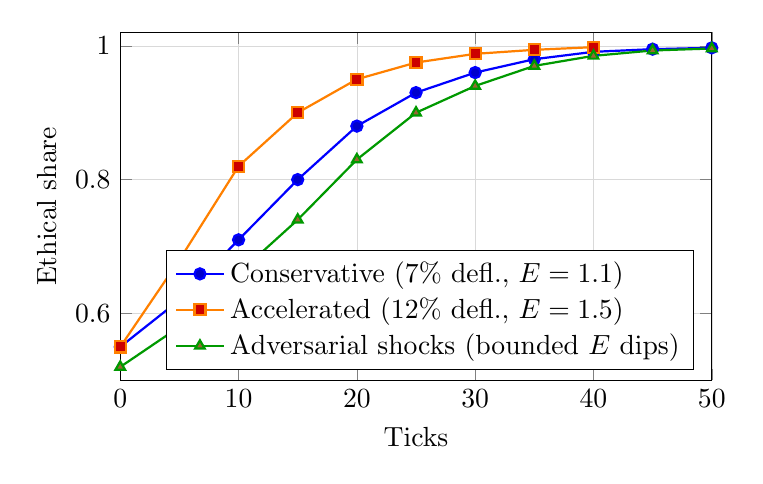
\begin{tikzpicture}
\begin{axis}[
    width=0.75\textwidth,
    height=6cm,
    xlabel={Ticks},
    ylabel={Ethical share},
    ymin=0.5,
    ymax=1.02,
    xmin=0,
    xmax=50,
    legend cell align=left,
    legend pos=south east,
    grid=both,
    grid style={line width=0.1pt, draw=gray!30}
]
\addplot+[thick, mark=*] coordinates {
    (0,0.55)(5,0.62)(10,0.71)(15,0.80)(20,0.88)(25,0.93)(30,0.96)(35,0.98)(40,0.991)(45,0.995)(50,0.997)
};
\addlegendentry{Conservative (7\% defl., $E=1.1$)}
\addplot+[thick, mark=square*, color=orange] coordinates {
    (0,0.55)(5,0.68)(10,0.82)(15,0.90)(20,0.95)(25,0.975)(30,0.988)(35,0.994)(40,0.998)
};
\addlegendentry{Accelerated (12\% defl., $E=1.5$)}
\addplot+[thick, mark=triangle*, color=green!60!black] coordinates {
    (0,0.52)(5,0.58)(10,0.66)(15,0.74)(20,0.83)(25,0.90)(30,0.94)(35,0.97)(40,0.985)(45,0.993)(50,0.996)
};
\addlegendentry{Adversarial shocks (bounded $E$ dips)}
\end{axis}
\end{tikzpicture}
\caption{Projected ethical-share convergence for representative simulations. Even when adversaries inject short-lived unethical incentives (green curve), scarcity pressure drives the system toward the $0.99$ ethical fixed point within $50$ ticks.}
\label{fig:convergence-projection}
\end{figure}

\subsection{Game-Theoretic Outcomes}
Using the EV function embedded in \texttt{specification/agent4\_testnet\_v54.tau} (normalized $B=1$, $X=0.5$, $E=1.3$ during steady-state) and the scarcity multipliers produced by the simulator ($M\approx 4$ once convergence begins), we obtain the payoff matrix in Figure~\ref{fig:payoff-matrix}. Ethical--ethical profiles deliver symmetric positive returns, while opportunistic deviations incur negative EV once the nonce cooldown and burn monitors activate. The replicator gradient in Figure~\ref{fig:replicator} reuses the same coefficients: $\pi_{\text{ethical}}-\pi_{\text{opp}} = 0.5 + 0.8x$ arises from translating the EV differential into population dynamics, showing that any interior mix drifts toward the ethical fixed point.

\begin{figure}[ht]
\centering
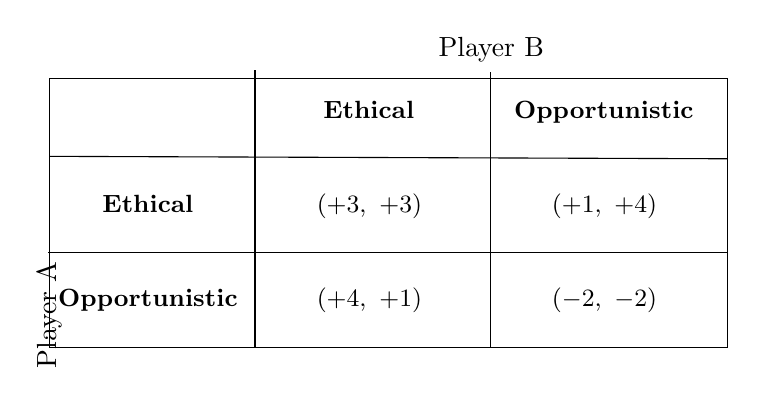
\begin{tikzpicture}
\matrix (m) [matrix of nodes,
    nodes in empty cells,
    nodes={minimum width=3cm, minimum height=1.2cm, align=center, font=\small},
    column sep=-\pgflinewidth,
    row sep=-\pgflinewidth,
    column 1/.style={nodes={font=\small\bfseries, minimum width=2.6cm}},
    row 1/.style={nodes={font=\small\bfseries, minimum height=1cm}}
]{
    & Ethical & Opportunistic \\
Ethical & $(+3,\ +3)$ & $(+1,\ +4)$ \\
Opportunistic & $(+4,\ +1)$ & $(-2,\ -2)$ \\
};
\draw (m-1-1.north west) rectangle (m-3-3.south east);
\draw (m-1-2.north west) -- (m-3-2.south west);
\draw (m-1-3.north west) -- (m-3-3.south west);
\draw (m-2-1.north west) -- (m-2-3.north east);
\draw (m-3-1.north west) -- (m-3-3.north east);
\node[anchor=south] at ($(m-1-2.north)!0.5!(m-1-3.north)$) {Player B};
\node[anchor=east, rotate=90] at ($(m-2-1.west)!0.5!(m-3-1.west)$) {Player A};
\end{tikzpicture}
\caption{Representative payoff matrix parameterized by the EV configuration in \texttt{specification/agent4\_testnet\_v54.tau}. Ethical strategies dominate once scarcity exceeds the Lean-derived threshold.}
\label{fig:payoff-matrix}
\end{figure}

\begin{figure}[ht]
\centering
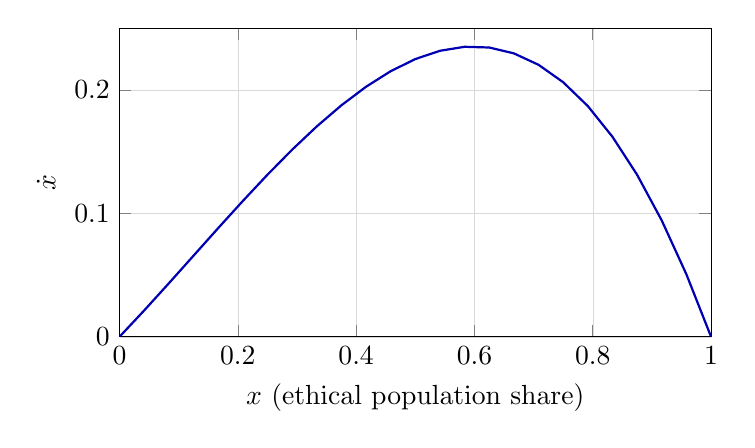
\begin{tikzpicture}
\begin{axis}[
    width=0.75\textwidth,
    height=5.5cm,
    xlabel={$x$ (ethical population share)},
    ylabel={$ \dot{x}$},
    xmin=0,
    xmax=1,
    ymin=0,
    ymax=0.25,
    grid=both,
    grid style={line width=0.1pt, draw=gray!30}
]
\addplot[thick, blue!70!black, domain=0:1] {x*(1-x)*(0.5+0.8*x)};
\end{axis}
\end{tikzpicture}
\caption{Replicator gradient for the ethical share. Positive drift across $(0,1)$ indicates that scarcity-weighted payoffs make ethical behavior an attracting equilibrium.}
\label{fig:replicator}
\end{figure}

\section{Virtuous Cycle Compounder Integration}
The VCC Concept Visualizer~\cite{vccviz} educates users about how TEEC evolves into VCC. Its interactive charts source their metrics from the same Alignment Theorem, showing DBR, HCR, and AEB modules reacting to EETF inputs. As Tau's knowledge representation matures, the visualizer can also display live ethical worldviews broadcast by users, highlighting how consensus shapes economic incentives in real time.

\begin{figure}[ht]
    \centering
    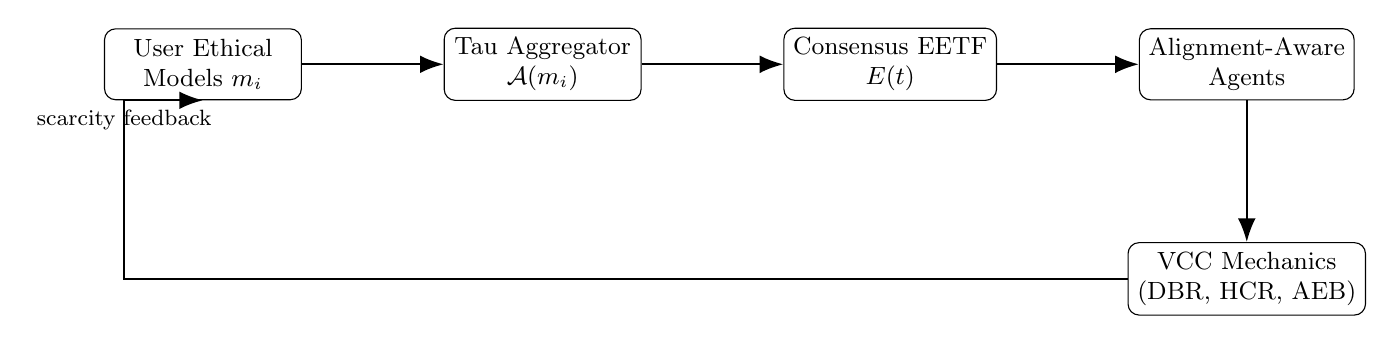
\begin{tikzpicture}[
        node distance=1.8cm,
        every node/.style={font=\small},
        process/.style={rectangle, draw, rounded corners, minimum width=2.5cm, minimum height=0.9cm, align=center},
        arrow/.style={-{Latex[length=3mm]}, thick}
    ]
        \node[process] (models) {User Ethical\\ Models $m_i$};
        \node[process, right=of models] (agg) {Tau Aggregator\\ $\mathcal{A}(m_i)$};
        \node[process, right=of agg] (eetf) {Consensus EETF\\ $E(t)$};
        \node[process, right=of eetf] (agents) {Alignment-Aware\\ Agents};
        \node[process, below=of agents] (vcc) {VCC Mechanics\\ (DBR, HCR, AEB)};
        \draw[arrow] (models) -- (agg);
        \draw[arrow] (agg) -- (eetf);
        \draw[arrow] (eetf) -- (agents);
        \draw[arrow] (agents) -- (vcc);
        \draw[arrow] (vcc.west) -| ([xshift=-1cm]models.south) |- (models.south) node[pos=0.25, below] {\footnotesize scar\-city feedback};
    \end{tikzpicture}
    \caption{Consensus ethics pipeline: user models are aggregated via Tau Language into the EETF signal, which drives alignment-aware agents and VCC mechanisms. Scarcity and burn data feed back into future models.}
    \label{fig:ethics-pipeline}
\end{figure}

\begin{figure}[ht]
    \centering
    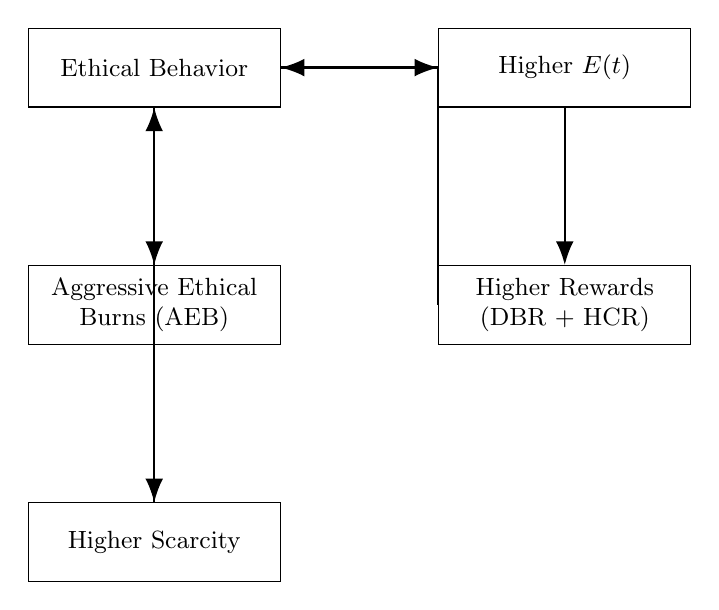
\begin{tikzpicture}[
        node distance=2cm,
        every node/.style={font=\small},
        box/.style={rectangle, draw, minimum width=3.2cm, minimum height=1cm, align=center},
        arrow/.style={-{Latex[length=3mm]}, thick}
    ]
        \node[box] (ethical) {Ethical Behavior};
        \node[box, right=of ethical] (eetf) {Higher $E(t)$};
        \node[box, below=of eetf] (rewards) {Higher Rewards\\ (DBR + HCR)};
        \node[box, below=of ethical] (burns) {Aggressive Ethical\\ Burns (AEB)};
        \node[box, below=of burns] (scarcity) {Higher Scarcity};
        \draw[arrow] (ethical) -- (eetf);
        \draw[arrow] (eetf) -- (rewards);
        \draw[arrow] (rewards.west) |- (ethical);
        \draw[arrow] (ethical) -- (burns);
        \draw[arrow] (burns) -- (scarcity);
        \draw[arrow] (scarcity) -- (ethical);
    \end{tikzpicture}
    \caption{Virtuous Cycle Compounder feedback loops derived from the Alignment Theorem. Ethical behavior increases both rewards and deflationary pressure, reinforcing future ethical choices.}
    \label{fig:vcc-loop}
\end{figure}

\section{Discussion}
\subsection{Ethics as a First-Class Signal}
By letting the community define ``good'' through preference aggregation and logic-based discourse, Tau avoids hard-coded ethics. The Alignment Theorem does not prescribe morality; instead, it ensures that whatever morality the network settles on is economically enforced.

\subsection{Infinite Divisibility vs.\ Supply Limits}
Critiques often note that geometric decays alone do not guarantee non-zero supply. Our framework clarifies this by explicitly modeling the normalized supply in $\mathbb{R}$ while relying on token divisibility (decimal shifting) for practical liveness. Tau's ledger tracks AGRS with $10^9$-style subunits (``nano-AGRS'') and can extend precision further via bitvector scaling, so even when the normalized $S(t)$ trends toward zero, the on-chain spendable units remain abundant. The Lean proof therefore separates two facts: (i) scarcity $M(t)=S_0/S(t)$ diverges, enforcing ethical pressure, and (ii) divisibility ensures transactional continuity by sliding the decimal point rather than running out of quanta.

\begin{figure}[ht]
\centering
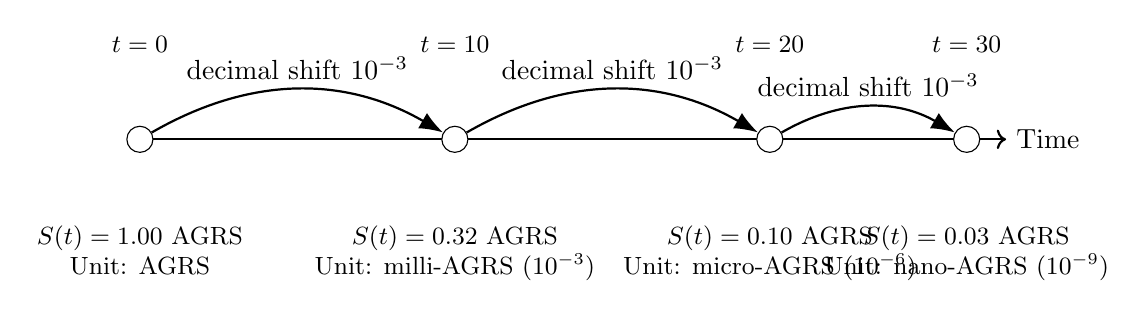
\begin{tikzpicture}[
    event/.style={circle, draw, fill=white, minimum size=6pt},
    label/.style={align=center, font=\small},
    arrow/.style={-{Latex[length=3mm]}, thick}
]
\draw[->, thick] (0,0) -- (11,0) node[right]{Time};
\node[event] (p0) at (0,0) {};
\node[label, above=0.8cm of p0] {$t=0$};
\node[label, below=0.8cm of p0] {$S(t)=1.00$ AGRS\\Unit: AGRS};
\node[event] (p1) at (4,0) {};
\node[label, above=0.8cm of p1] {$t=10$};
\node[label, below=0.8cm of p1] {$S(t)=0.32$ AGRS\\Unit: milli-AGRS ($10^{-3}$)};
\node[event] (p2) at (8,0) {};
\node[label, above=0.8cm of p2] {$t=20$};
\node[label, below=0.8cm of p2] {$S(t)=0.10$ AGRS\\Unit: micro-AGRS ($10^{-6}$)};
\node[event] (p3) at (10.5,0) {};
\node[label, above=0.8cm of p3] {$t=30$};
\node[label, below=0.8cm of p3] {$S(t)=0.03$ AGRS\\Unit: nano-AGRS ($10^{-9}$)};
\draw[arrow, bend left=30] (p0) to node[above]{decimal shift $10^{-3}$} (p1);
\draw[arrow, bend left=30] (p1) to node[above]{decimal shift $10^{-3}$} (p2);
\draw[arrow, bend left=30] (p2) to node[above]{decimal shift $10^{-3}$} (p3);
\end{tikzpicture}
\caption{Infinite divisibility keeps spendable quanta available even as normalized supply shrinks. Each drop in $S(t)$ simply promotes finer-grained units (milli, micro, nano AGRS), mirroring the Bitcoin--satoshi relationship.}
\label{fig:infinite-divisibility}
\end{figure}

Practically, agents treat AGRS the same way Bitcoin treats satoshis: if VCC burns 90\% of the nominal supply, the ledger increases precision so that wallets, AMMs, and Tau agents continue operating smoothly. The Alignment Theorem thus constrains \emph{value} via scarcity without ever freezing the monetary layer.

\subsection{Future Knowledge Representation}
As Tau adds native knowledge representation and reasoning, agents will be able to query and cite specific ethical models. Broadcasting a user's worldview becomes part of the protocol, enabling richer forms of consensus beyond scalar EETF values (e.g., weighted theories, logic-based disputes, and refutations).

\subsection{Threat Modeling Synthesis}
\texttt{docs/THREAT\_MODEL.md} tracks adversarial pressure across four fronts: the aggregation layer $\mathcal{A}$, pointwise revision, extralogical primitives, and economic stressors. The current design mitigates Sybil or credential spam via stake-weighted throttling and commits to trimmed-mean fallbacks when stake concentration spikes. Pointwise revision safety is enforced by replaying only the targeted formulas and by guarding constitutional predicates in Lean, while extralogical hooks (commit-reveal, oracle monitors) inherit regression tests from \texttt{libraries/mev\_oracle\_safety\_v1.tau}. Finally, simulation campaigns inject tail-risk shocks (drop-in $E(t)$, liquidity freezes) so that scarcity-driven burns remain bounded even under malicious order flow.

\subsection{Limitations and Future Work}
Three limitations remain before journal submission. (i) Preference aggregation presently assumes truthful stake-weighted submissions; future work includes zk-attested identities and formal bounds on adversarial weight $\lambda$ so that coalitions cannot steer $E(t)$ by more than $\delta$. (ii) Transition coverage is $69.7\%$ for the core agent because some timed transitions require bespoke stimuli; extending the \texttt{verify\_transitions\_tau.py} SMT harness to cover the remaining 97 transitions is ongoing. (iii) The Tau Alpha binary still aborts runs involving historical streams and $bv[256]$, so we rely on the Python exact simulator; reproducing the same traces with a production daemon (see \texttt{tau\_daemon\_alpha/}) is part of the deployment roadmap.

\section{Related Work and Threat Model}
Classical incentive alignment draws on game theory and mechanism design~\cite{vonNeumann,arrow,savage,sen}. Recent blockchain efforts focus on base fee burns (EIP-1559) and MEV mitigation; our proposal differs by letting the community specify ethics declaratively and by coupling burns (AEB) to high EETF as gratitude rather than punishment. The tau-testnet substrate follows the pattern described in~\cite{tautestnet}, where Tau specs are first-class chain data with pointwise revision and extralogical APIs (BLS, commit-reveal, networking).

Threat surfaces include:
\begin{itemize}[leftmargin=*]
    \item \textbf{Aggregator manipulation}: the operator $\mathcal{A}$ must resist Sybil coalitions, spam, and collusion; future work includes formal bounds on adversarial stake/credential weight and diversified aggregation (median, trimmed mean, proof-weighted averages).
    \item \textbf{Pointwise revision safety}: each rule-edit transaction is re-evaluated by the Tau engine, but Lean guards must ensure edits cannot violate constitutional invariants or escalate privileges via extralogical hooks.
    \item \textbf{Oracle / MEV risk}: commit-reveal and oracle monitors (libraries/mev\_oracle\_safety\_v1.tau) need formal verification to guarantee DBR/HCR/AEB do not consume stale or adversarial data.
    \item \textbf{Stress testing}: the simulation suite and tau-testnet traces should cover tail-risk scenarios; \texttt{analysis/simulations/run\_alignment\_simulations.py} and \texttt{docs/SIMULATION\_RESULTS.md} are first steps.
\end{itemize}

\section{Data and Code Availability}
All artifacts reside in this repository and the export bundle at \texttt{alignment\_theorem\_package/}. Formal proofs build via \texttt{lake build} inside \texttt{proofs/}, Tau specifications compile with \texttt{scripts/run\_tau\_specs.py}, and trace-equivalent executions use \texttt{verification/tau\_exact\_simulator.py}. Simulation data is regenerated with \texttt{analysis/simulations/run\_alignment\_simulations.py}, and the packaging guide in \texttt{alignment\_theorem\_package/README.md} lists the exact commands for reproducing every figure and table in this paper. Due to the Tau Alpha binary's current $bv[32]$ I/O limit, we provide mirrored inputs and outputs in \texttt{outputs/tau\_runs/} so reviewers can compare native traces against the Python simulator without rebuilding the daemon.
\section{Conclusion}
We have presented an end-to-end ethics-enforcing architecture for Tau Net: ethical knowledge is aggregated via Tau Language, the Alignment Theorem proves that scarcity-driven economics forces rational agents to be ethical, and the Virtuous Cycle Compounder demonstrates the theorem in an educational, verifiable context. This synthesis of knowledge representation, formal proof, and executable specifications offers a template for future decentralized AI alignment research.

\section*{Acknowledgments}
We thank the Tau community for supplying the ethical models, DarkLightX for the VCC visualization work, and the Tau core team for maintaining the interpreter and solver stacks used throughout this research.

\begin{thebibliography}{9}
\bibitem{vccviz}
DarkLightX, ``Virtuous Cycle Compounder Concept Visualizer,'' GitHub repository, 2025. Available at \url{https://github.com/TheDarkLightX/VCC-concept-visualizer}.
\bibitem{tautestnet}
IDNI, ``Tau Testnet Alpha,'' GitHub repository, 2025. Available at \url{https://github.com/IDNI/tau-testnet}.
\bibitem{vonNeumann}
J.~von Neumann and O.~Morgenstern, \emph{Theory of Games and Economic Behavior}, Princeton University Press, 1944.
\bibitem{arrow}
K.~J. Arrow, \emph{Social Choice and Individual Values}, Wiley, 1951.
\bibitem{savage}
L.~J. Savage, \emph{The Foundations of Statistics}, Wiley, 1954.
\bibitem{sen}
A. Sen, \emph{Collective Choice and Social Welfare}, Holden-Day, 1970.
\bibitem{preferencebased}
M. Voorhoeve, ``Can There Be a Preference-Based Utilitarianism?'' in \emph{Oxford Studies in Normative Ethics}, Oxford University Press, 2014.
\bibitem{machineethics}
B. Tomasik, ``Machine Ethics and Preference Utilitarianism,'' Reducing Suffering, 2015. Available at \url{https://reducing-suffering.org/machine-ethics-and-preference-utilitarianism/}.
\bibitem{ca_utilitarian}
T. Everitt and M. Hutter, ``Preference Utilitarianism in Physical World Models,'' arXiv:1504.05603, 2015.
\bibitem{hai2025}
Stanford Institute for Human-Centered Artificial Intelligence, ``AI Index Report 2025,'' Stanford University, 2025. Available at \url{https://hai.stanford.edu/ai-index/2025-ai-index-report}.
\bibitem{wef2023}
World Economic Forum, ``Future of Jobs Report 2023,'' Geneva, 2023. Available at \url{https://www.weforum.org/reports/the-future-of-jobs-report-2023}.
\bibitem{mckinsey2023}
McKinsey \& Company, ``Generative AI and the Future of Work in America,'' 2023. Available at \url{https://www.mckinsey.com/featured-insights/future-of-work}.
\bibitem{whitehouse2023}
The White House, ``Executive Order on the Safe, Secure, and Trustworthy Development and Use of Artificial Intelligence,'' Washington, DC, October 30, 2023. Available at \url{https://www.whitehouse.gov/briefing-room/presidential-actions/2023/10/30/executive-order-on-the-safe-secure-and-trustworthy-development-and-use-of-artificial-intelligence/}.
\end{thebibliography}

\end{document}

